\chapter{Future Work}
\label{cha:future_work}

Although Whisker is usable in its current form,
there are still many opportunities to improve it in the future.
\parspace

\textbf{Automated input.}
While Whisker's automated input algorithm works quite well, it is still very simple.
One could use more elaborate static analysis or search-based techniques to find better fitting inputs.
For example, sequences of input may be found, and the optimal duration and probability of a key press or a sequence may be determined.
At the same time, the algorithm may construct correct answers to \texttt{ask} blocks at run time.
Figure~\ref{fig:generated_ask_answer} shows an ask-answer configuration from one of Code Club's sample solutions,
for which answers may be generated.

\begin{figure}[htpb]
    \centering
    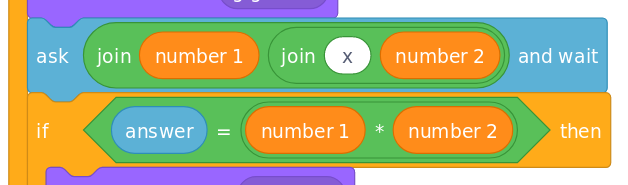
\includegraphics[width=0.4\textwidth]{scratch-ask-answer}
    \caption{Ask-answer configuration with a generated question and answer}
    \label{fig:generated_ask_answer}
\end{figure}


\textbf{Simplify tests with helper methods.}
Tests with Whisker can quickly become quite long and complex.
Therefore, Whisker should should provide more features that simplify writing tests.
One task, which currently requires a large amount of code,
is checking temporal relationships between two events,
for example ''one second after some sprite touches a border, some variable must be increased''.
In the future, testing may be simplified greatly by providing methods to handle cases like this.
\parspace

\textbf{Support for audio and Scratch extensions.}
Whisker could be extended to support sounds and Scratch extensions.
Scratch has a small number of extensions, which add blocks with various functionality.
For example, the \textit{Pen} extension allows to freely draw on the stage by controlling a pen through the program,
and the \textit{Video Sensing} extensions allows to detect movement with a web cam.
Adding support for audio as well as extensions in the future would make Whisker applicable to a wider range of Scratch projects.
\parspace

\textbf{User interface.}
Another thing to improve, is Whisker's user interface.
Currently Whisker only has a web GUI, which is accessed through a web browser.
This interface can be used to test projects in batch, but it still requires manual user interaction to select programs and tests,
and to save the test report once the test execution finished.
In the future, a standalone Electron~\cite{electron} application could solve these problems by allowing Whisker to directly load projects and tests,
and to directly save test reports.
It would also make it possible to run tests in parallel more easily.
\parspace

\textbf{Seeding randomness.}
Non-deterministic programs can be problematic for testing since the behaviour of such programs may change from one execution to another.
This is especially problematic for faulty implementations.
Bugs may only sometimes cause incorrect behaviour, causing inconsistent test outcomes.
This may be avoided by seeding the random number generator so it produces the same random numbers for each program execution.



